\chapter{Modèles}
\label{chap:Modeles}

\section{Choix des modèles}
Le choix des modèles a été un choix rapide.\newline
Nous avons commencé par regarder les tutoriels sur les sites web des frameworks que nous utilisons. Nous avons donc regardé les tutotiels de pytorch, car nous voulions utiliser ce framework en particulier, mais avons aussi regardé les githubs de modèles dont nous avions entendu parler, comme YOLOv5. Il faut noter que notre compréhension du problème et du jargon utilisé dans le domaine s’est enrichi au fur et à mesure de nos recherches. \newline 
Ainsi, nos premiers choix peuvent sembler mauvais, mais lors de la prise de décision nous étions persuadés de faire les bons choix. Notre approche de départ se basait essentiellement sur un facteur: nous voulions des modèles pour lesquels il existe beaucoup de ressources en ligne. Cette méthodologie nous a amené à explorer une solution (YOLOv5) qui n’était pas adaptée à notre problème. \newline
Après beaucoup d’essais infructueux, nous avons donc changé de méthodologie et nous nous sommes laissé la liberté d’utiliser des outils de plus haut niveau, tel que Detectron2 et de ne pas se restreindre uniquement à PyTorch. Une fois que nous avons pris en main ce framework, nous avons pu nous concentrer sur la performance du modèle. C'est aussi à ce stade que nous avons compris que le score sur le benchmark COCO2017 indiqué sur beaucoup de documentation de modèles était justement indiqué pour pouvoir comparer les modèles entre eux.

\section{Les échecs}
\subsubsection{YOLOv5}
YOLO est l'acronyme de You Only Look Once; il s'agit du premier modèle que nous avons essayé. Nous avons décidé de commencer avec ce modèle pour plusieurs raisons parmi lesquelles : une abondance de tutoriels sur le net et une solution qui nous semblait clé en main pour résoudre notre problème. Malgré ces signes positifs, il n’a pas été une solution adaptée. \newline
En effet, YOLO, a été publié il y a plusieurs année et n’est plus forcément l’état de l’art actuel. De plus, ce modèle est adapté à du traitement en temps réel ce qui ne fait pas partie de notre problème. Cependant, le réel souci qui nous a fait abandonner cette solution est la structure spéciale du dataset qui ne correspondait pas à notre structure. \newline 
Durant une phase de réflexion visant à résoudre le souci de structure, nous avons ainsi réalisé l’incapacité du modèle à gérer des images n’étant pas de 640x640 pixels. Nous aurions pu effectuer un réajustement de la taille des images mais ces derniers éléments nous ont fait réaliser que YOLO n’était pas la solution clé à laquelle nous nous attendions et avons décidé après quelques discussions de passer à un modèle plus adapté à notre problème initial. C'est ainsi que nous nous sommes lancé sur faster R-CNN, un modèle qui supporte des images de tailles arbitraires et qui est plus récent que YOLOv5.

\subsubsection{SSD}
\paragraph{} L'object detection étant une application nouvelle pour nous quand nous débutions le projet, après l'échec du modèle YOLO, nous avons décidé de nous lancer en parallèle sur différents modèles, le but étant de trouver celui ou ceux pouvant répondre efficacement à notre problématique. C'est dans cette optique que nous avons exploré le modèle SSD (Single Shot Multibox Détector). C'est un algorithme de detection d'objet dans une image qui au moment de la prédiction, divise l’image à l’aide d’une grille et génère des scores pour la présence de chaque catégorie d'objet dans chaque grille par défaut puis ajuste la grille pour mieux correspondre à la forme de l'objet. Le réseau combine ainsi les prédictions de plusieurs cartes de caractéristiques avec différentes résolutions pour traiter naturellement des objets de tailles diverses. Ce réseau se veut d'après la documentation, plus rapide que YOLO et aussi précis que FasterRCNN. 
\paragraph{} Nous avons trouvé un exemple d'implémentation sur \url{https://pytorch.org/hub/nvidia_deeplearningexamples_ssd}. La mise en oeuvre de celui ci s'est faite sans trop de douleur. Par la suite, il était question de faire du transfert learning ou fine tuning selon les documents. En effet, le modèle a été entrainé sur le dataset COCO (MS COCO: Microsoft Common Objects in Context) qui est un jeu de données d'images à grande échelle contenant 328 000 images d'objets quotidiens et d'êtres humains. Nous souhaitons donc ré-entrainer une partie du réseau avec notre set d'images. Pour ce faire nous nous sommes aidé d'un tutoriel trouvé sur git à l'adresse \url{https://github.com/Coldmooon/SSD-on-Custom-Dataset}. Dans celle ci est expliqué une façon d'entrainer le modèle SSD sur un dataset personnalisé avec pour contrainte que les images doivent être de taille 300*300 ou 512*512. Travailler sur des images carrées était l'un des problèmes que nous avons rencontré avec YOLO, mais nous avons pensé résoudre ce problème avec les fonctions de resizing existantes. 
Nous avons ccommencé par éssayer de reproduire le tuto sur le dataset proposé dans celui-ci. A de nombreuses reprises, nous avons fait face à des erreurs dont nous ignorions la provenance ainsi que la solution. Pour finir cela nous a pris beaucoup de temps pour au final ne pas arriver à entrainer le modèle sur le dataset en question. Nous n'avons donc pas pu aller au bout de cette implémentation. Mais nous restons convaincus que ça reste une alternative à la résolution de notre problématique.

\subsubsection{Faster R-CNN avec Keras}

\paragraph{} Après l'échec de YOLOv5 en raison de la nécessité d'utiliser des images carrées de taille fixe, nous avons décidé de nous pencher sur une utilisation potentielle d'un réseau de neurones de type Faster R-CNN, plus précisément en utilisant la bibliothèque open-source Keras puisque c'est une bibliothèque que nous avions déjà utilisée auparavant dans le cadre du cours sur les réseaux de neurones. Pour atteindre cet objectif, nous avions à disposition une implémentation toute faite de Faster R-CNN utilisant Keras disponible à l'adresse suivante : \url{github.com/you359/Keras-FasterRCNN}. Malheureusement, nous avons rencontré un certain nombre de problèmes au moment d'utiliser l'implémentation fournie.

\paragraph{} Tout d'abord, il s'agit d'un code plutôt ancien qui n'est pas forcément compatible avec les dernières versions des librairies utilisées en Python. En effet, ces librairies sont régulièrement mises à jour et certaines fonctions disponibles sont alors dépréciées, modifiées voire même définitivement supprimées. Il a donc fallu trouver par tâtonnement les bonnes versions des librairies à utiliser en créant de multiples environnements virtuels à l'aide de conda et en intérprétant les divers messages d'erreur énigmatiques renvoyés à chaque nouvelle tentative. Finalement, nous avons réalisé que le repo github contenait un fichier texte indiquant les versions optimales des librairies à utiliser pour ce projet. Cependant, même en utilisant les versions recommandées, le code continuait à planter après quelques secondes pour d'obscures raisons.

\paragraph{} Ensuite, le second problème réside dans la documentation de l'implémentation de Faster R-CNN qui contient ce qui semble être une grossière erreur quant à la version de Python à utiliser. En effet, nous avons appris au point précédent qu'il valait mieux lire attentivement la documentation disponible avant de se lancer corps et âme dans le code. Or cette documentation indique explicitement d'utiliser Python 2 pour faire tourner le code mis à disposition. Malheureusement, même en utilisant les bonnes versions des librairies et de python le code ne voulait définitivement pas fonctionner. Dans une tentative désespérée nous avons donc changé la version de Python pour Python 3 et là, comme par magie, le code commence à tourner et le réseau de neurones commence à s'entraîner.

\paragraph{} Finalement, nous arrivons au problème principal que nous n'avons jamais réussi à résoudre et qui est donc la raison pour laquelle nous avons abandonné ce modèle. En effet, même si le code parvenait désormais à se lancer correctement, il plantait maintenant à des étapes aléatoires de l'entraînement du réseau de neurones, parfois après quelques secondes, parfois après quelques dizaines de minutes, mais toujours en renvoyant une grande quantité de messages d'erreur pratiquement incompréhensibles. Malgré de longues et intenses recherches sur de mutliples sites internet et forums, personne ne semblait en mesure de trouver une solution à ce problème. En effet, d'autres utilisateurs rencontraient le même souci mais la solution adoptée au final était toujours la même : changer de modèle, souvent pour passer sur detectron qui possède une documentation beaucoup plus complète, ce que nous avons donc également fait par la suite. Nous avons tout de même réussi à finir un entraînement sans encombre, mais pour y parvenir il a fallu réduire drastiquement le nombre d'epochs afin de limiter la durée de l'entraînement, et à la fin de celui-ci le réseau de neurones n'était pas capable de reconnaître quoi que ce soit sur les images, probablement en raison du manque d'entraînement.

\paragraph{} Pour conclure, on peut donc dire que le coeur du problème de l'implémentation utilisée est son manque de popularité dans la communauté du data science. En effet, comme les utilisateurs sont peu nombreux, des erreurs se glissent dans la documentation et passent inaperçues tandis que d'autres problèmes restent à jamais non-résolus car personne ne semble connaître la solution. Nous avons donc choisi d'utiliser par la suite des modèles plus populaires et par conséquent mieux documentés. 

\section{Les réussites}

\subsection{Detectron2}
Detectron2 est une puissante plateforme de détection d'objets et de segmentation d'images développée par Facebook AI Research (FAIR). Il s'agit de la deuxième génération du système Detectron original, également développé par FAIR. Detectron2 est conçu pour être hautement modulaire et flexible, et il est utilisé pour un large éventail de tâches de computer vision, comme la détection d'objets, la segmentation d'instances, la segmentation panoptique, et plus encore. Il est construit au-dessus du framework PyTorch et présente une variété de modèles de pointe. L'utiliser nous a permis de facilement changer de modèle une fois que notre code d'entrainement était fonctionnel.
En effet, beaucoup de configuration se font à travers le fichier de configuration, c'est dans lui qu'on spécifie les détails du processus d'entrainements tels que le set de données d'entrainement, le set de validation, le modèle à entrainer, le learning-rate etc. De plus, il intégre de nombreuses configuration de bases et grâce à ceci nous n'avons qu'à changer les paramètres qui nous intéressent comme : la backbone du modèle, les poids à charger pour faire du transfert learning. Detectron2 intégre directement dans la class \verb|DefaultTrainer| une méthode qui affiche des statistiques sur l'entrainement en cours, comme le nombre d'epochs, le learning-rate, le temps restant, etc. Cela nous a permis de suivre l'entrainement de nos modèles. Il s'occupe aussi de faire de l'augmentation de données durant le processus d'entrainement. Finalement, Detectron2 fournit aussi pour tous ses modèles des poids après entrainement du modèle.
\paragraph{}
Entrainer un modèle avec Detectron2 se résume donc à faire un code similaire à celui visible en ci-dessous.
\lstset{style=Python}
\begin{lstlisting}
from detectron2 import model_zoo
from detectron2.engine import DefaultPredictor
from detectron2.config import get_cfg
cfg = get_cfg()
# On charge une configuration de base
cf_file="COCO-Detection/faster_rcnn_X_101_32x8d_FPN_3x.yaml"
cfg.merge_from_file(model_zoo.get_config_file(cf_file))
cfg.DATASETS.TRAIN = ("triton_train",)
cfg.MODEL.WEIGHTS = model_zoo.get_checkpoint_url(cf_file)  
# cfg.params... voir dans la documentation
trainer = DefaultTrainer(cfg) 
trainer.resume_or_load(resume=False)
trainer.train()
predictor = DefaultPredictor(cfg)
\end{lstlisting}
\paragraph{}
En conclusion Detectron2, nous avons a permis de facilement changer de modèle et de tester plusieurs modèles. Nous avons aussi pu facilement faire du transfert learning en chargeant les poids d'un modèle pré-entrainé. 


\subsection{FASTER R-CNN}

Le modèle d'apprentissage automatique Faster R-CNN (R-CNN pour "Region-based Convolutional Network") vient à la base du modèle R-CNN, qui a été ensuite amélioré pour former le modèle Fast R-CNN, qui a lui-même finalement été optimisé pour créer le modèle Faster R-CNN étudié ici. R-CNN, Fast R-CNN et Faster R-CNN sont tous des modèles de traitement de l'image utilisés pour la détection d'objets dans les images. Ils utilisent tous une approche en plusieurs étapes qui consiste à extraire des caractéristiques de l'image à l'aide d'un réseau de neurones convolutionnel (CNN), puis à identifier les régions de l'image qui pourraient contenir des objets à l'aide de la sélection de région d'intérêt (ROI) et enfin à prédire la classe de chaque région sélectionnée et à localiser l'objet dans l'image.

\paragraph{R-CNN} est un modèle datant de 2014, dont on peut voir l'article scientifique \href{https://arxiv.org/pdf/1311.2524.pdf}{\textit{ici}}. Voici premièrement son architecture en figure \ref{fig:rcnn_architecture} ci-dessous.

\begin{figure}[H]
    \centering
    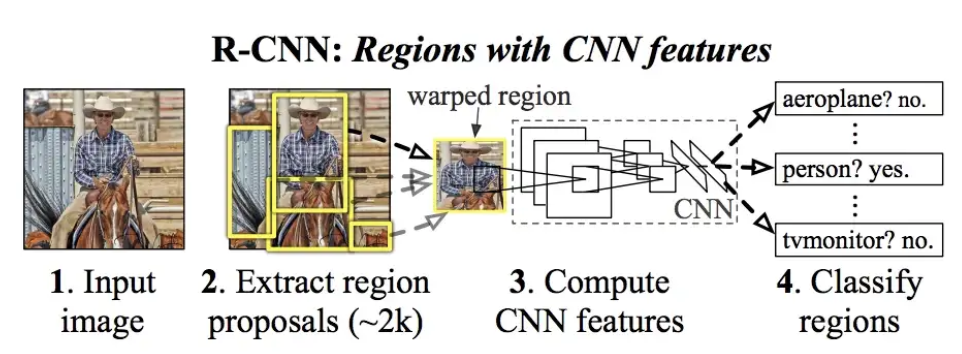
\includegraphics[width=300px]{images/model_rcnn_architecture.png}
    \caption{Architecture de R-CNN}
    \label{fig:rcnn_architecture}
\end{figure}

Comme dit précédemment, il s'agit du modèle original. Il est très performant, mais aussi très lent, car il traite chaque région sélectionnée de manière indépendante et entraîne un modèle de classification séparé pour chaque région.

% ---

\paragraph{Fast R-CNN} date d'une année plus tard, soit de 2015. On trouve son article scientifique \href{https://arxiv.org/pdf/1504.08083.pdf}{\textit{ici}} et voici son architecture en figure \ref{fig:fastRcnn_architecture} ci-dessous.

\begin{figure}[H]
    \centering
    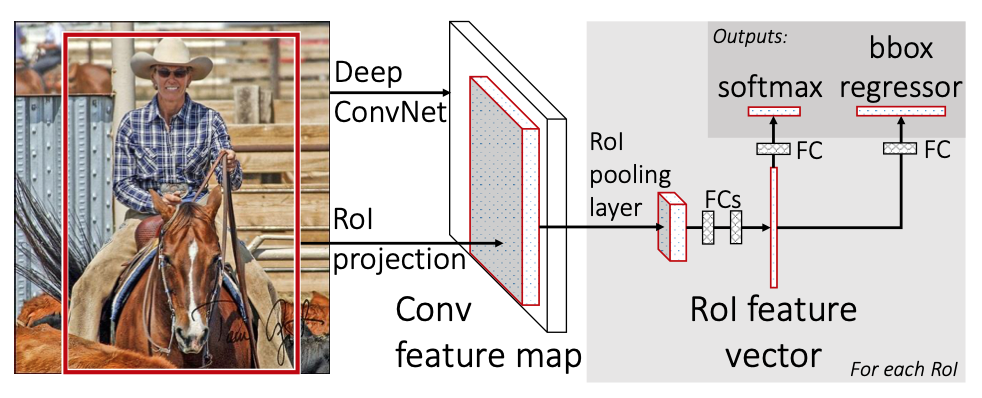
\includegraphics[width=250px]{images/model_fastRcnn_architecture.png}
    \caption{Architecture de Fast R-CNN}
    \label{fig:fastRcnn_architecture}
\end{figure}

Fast R-CNN est ainsi une version améliorée de R-CNN, qui est beaucoup plus rapide. Au lieu de traiter chaque région sélectionnée de manière indépendante, Fast R-CNN utilise un seul modèle de classification pour toutes les régions sélectionnées dans l'image. De plus, il utilise une technique appelée "max pooling régional" pour réduire la dimension des régions sélectionnées avant de les passer au modèle de classification.

% ---

\paragraph{Faster R-CNN} vient une année plus tard, en 2016.  \href{https://arxiv.org/pdf/1506.01497.pdf}{\textit{Ici}} se trouve son article scientifique, et voici finalement son architecture ci-dessous, en figure \ref{fig:fasterRcnn_architecture}.

\begin{figure}[H]
    \centering
    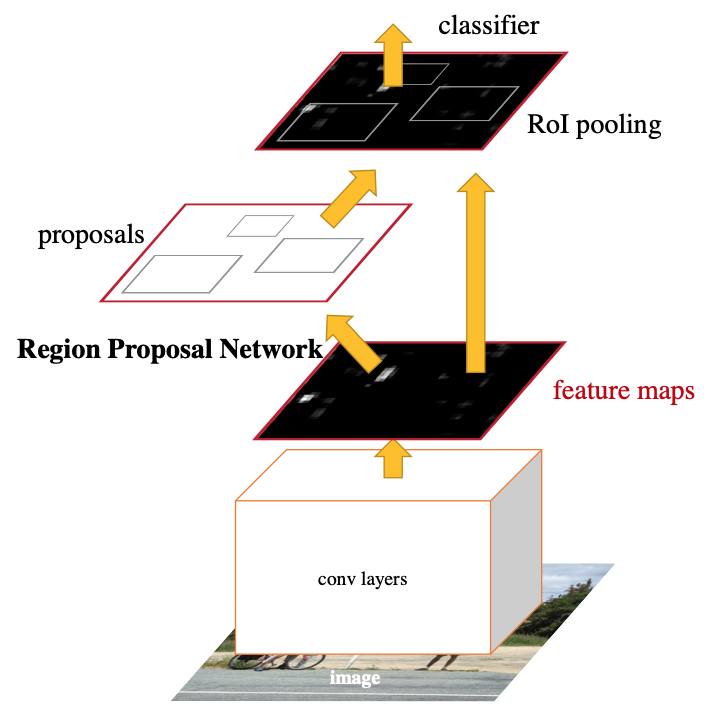
\includegraphics[width=250px]{images/model_fasterRcnn_architecture.png}
    \caption{Architecture de Faster R-CNN}
    \label{fig:fasterRcnn_architecture}
\end{figure}

\paragraph{} Faster R-CNN est effectivement un modèle encore plus rapide que Fast R-CNN. Il utilise une technique appelée "réseau de proposition de région" (RPN) pour identifier automatiquement les régions de l'image qui pourraient contenir des objets, sans avoir besoin de calculer explicitement toutes les régions de l'image comme le font R-CNN et Fast R-CNN. Cela permet à Faster R-CNN de traiter l'image de manière beaucoup plus rapide et de détecter des objets avec une précision comparable à celle de Fast R-CNN.

\paragraph{} Nous avons décidé d'utiliser une backbone \verb|X_101_32x8d_FPN| c'est à dire un réseau ResNeXt-101 avec une configuration de 32 groupes de large de 8, 32x8d fait donc référence à des hyper-paramètres utilisé par le réseau ResNeXt de la backbone. Nous n'avons pas nous même cherché ces valeurs, nous avons choisis cette configuration en copiant la configuration de Faster-RCNN donnant le meilleur score COCO selon la documentation de Detectron2. Ce réseau ResNeXt est suivit d'un second réseau, FPN cette fois, qui forment ensemble l'entièreté de la backbone que nous utilisons.

\paragraph{} Pour des raisons évidentes de rapidité de traitement des images, nous avons donc investigué plus précisément ce dernier modèle - Faster R-CNN - pour notre problème. C'est d'ailleurs ce modèle que nous avons finalement sélectionné pour répondre à la problématique de ce projet, comme mentionné ci-après, en chapitre \autoref{chap:Evaluation} de ce rapport ("Evaluation").\newline
Pour se faire, nous avons donc du adapter les exemples trouvés sur internet à notre problème, légèrement différent de ces dits exemples. Il a donc fallu assembler différents tutoriels, ce qui a impliqué beaucoup de temps d'analyse et de compréhension. Aussi, nous avons du nous habituer au jargon technique que nous n'avions pas - tel que mAP et les benchmarks coco pour en citer quelques uns. Il a également fallu passer du temps pour comprendre ce qu'était COCO (Common Object in COntext) : une base de données fournie par Microsoft qui contient des images annotées avec des informations sur les objets présents dans chaque imag et qui fourni également un benchmark ; un ensemble de tests et de métriques utilisés pour évaluer les performances des modèles de reconnaissance d'objets et de segmentation d'images.

% ------------------------------------------

\subsection{RETINA net}

\paragraph{Description}

\paragraph{} RetinaNet est un réseau de neurones convolutionnel utilisé en détection d'objets dans des images. Il a été présenté dans le papier "Focal Loss for Dense Object Detection" de Tsung-Yi Lin et al. en 2017.

\paragraph{} Le principe de base de RetinaNet est de prédire des scores de confiance pour chaque classe d'objet à chaque position de l'image, ainsi qu'une boîte englobante pour chaque objet détecté. Pour cela, RetinaNet utilise une architecture de réseau de neurones à deux branches, l'une pour prédire les scores de confiance et l'autre pour prédire les boîtes englobantes.

\paragraph{} La particularité de RetinaNet est qu'il utilise une "perte focale" pour lutter contre l'asymétrie des données dans les jeux de données de détection d'objets. Dans ces jeux de données, il y a souvent beaucoup plus de fond (c'est-à-dire des parties de l'image qui ne contiennent pas d'objets) que d'objets détectables. Cette asymétrie peut rendre difficile l'apprentissage pour le modèle, car il y a moins d'exemples d'objets à apprendre. La perte focale atténue cet effet en diminuant la contribution des exemples faciles (c'est-à-dire ceux où l'objet est facilement identifiable) à la perte totale, ce qui permet au modèle de se concentrer davantage sur les exemples difficiles.

\paragraph{} Le modèle RetinaNet est souvent utilisé dans les tâches de détection d'objets pour améliorer la précision et réduire le nombre de faux positifs. Il a été largement utilisé dans de nombreuses applications, notamment la reconnaissance de la circulation routière et la reconnaissance de la faune.

\paragraph{} Nous avons décidé d'utiliser une backbone \verb|R_101_FPN| c'est à dire un réseau ResNet-101 suivit d'un réseau FPN. Il s'agit selon la documentation de Detectron2 de la backbone qui donne un modèle RetinaNet le plus précis, c'est à dire donnant le meilleur score sur le benchmark COCO. Nous avons donc choisi ce modèle pour avoir un modèle précis et qui puisse être utilisé pour répondre à notre problématique de base.

\paragraph{} En résumé, RetinaNet est un modèle de détection d'objets qui utilise une architecture à deux branches et une perte focale pour améliorer la performance de détection dans les jeux de données asymétriques.

\paragraph{Results}

\paragraph{} Ce modèle obtient des résultats extrêmement satisfaisants. En effet, il s'agit du modèle qui détecte les crapauds/grenouilles avec la plus grande accuracy. Les résultats précis de ce modèle sont par ailleurs détaillés dans la section "Evaluation" du \autoref{chap:Evaluation} de ce rapport.

\subsection{\textit{De}tection \textit{Tr}ansformer (\textit{DE-TR)}}

\href{https://github.com/facebookresearch/detr}{DETR} est un modèle sorti en 2020 qui est extrêmement simple à implémenter et fournit des scores (mAP, IoU etc) sur le benchmark COCO qui surpassent ceux des modèles existants de quelques points. C’est pourquoi, en plus de son architecture innovante, nous avons voulu l’essayer. L’architecture, visible en figure \ref{fig:detr_architecture}, se base sur un transformer, un modèle de deep learning parut dans le fameux papier de 2017 de Google, \href{https://arxiv.org/pdf/1706.03762.pdf}{\textit{Attention is all you need}}. On peut observer que le modèle commence par générer des features à partir de l'image d'entrée en utilisant une backbone, c'est-à-dire un modèle pré-entrainé visant justement à extraire ces features à l'aide d'un réseau neuronal convolutif. Ensuite, le modèle utilise la partie encodeuse du transformer suivi de son équivalent décodeur et finalement d'un "prediction feed-forward networks" (FFN). C'est le réseau FFN qui génère les possibles bounding boxes et les classes associées.

\begin{figure}[th!]
    \centering
    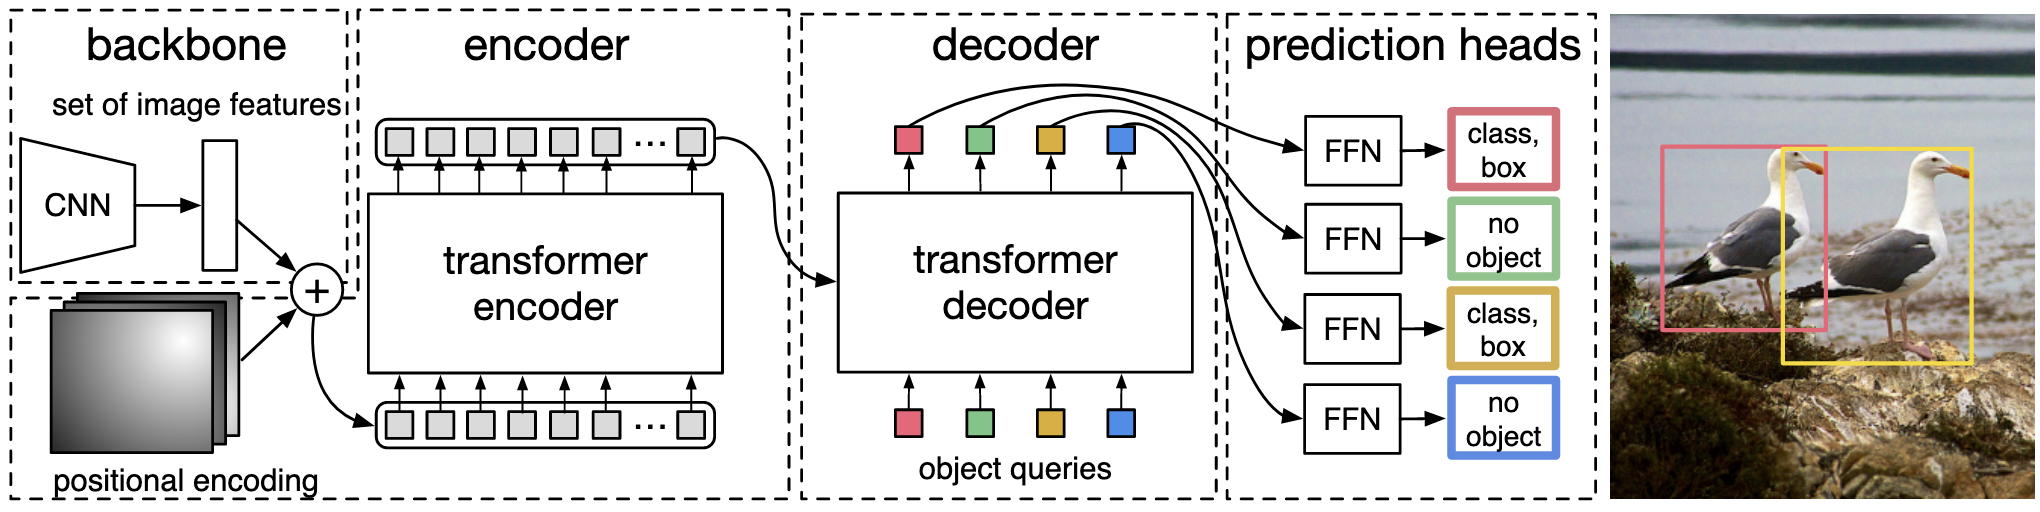
\includegraphics[width=\textwidth]{images/detr_architecture.png}
    \caption{Architecture de DETR}
    \label{fig:detr_architecture}
\end{figure}
% ----------------------------------------------------
Ce modèle est simple car il utilise peu de couches contrairement à FasterRCNN par exemple. Une implémentation PyTorch est faisable en 60 lignes. Cependant, l'entrainement est complexe et nous nous y sommes repris plusieurs fois pour réussir un entrainement.
DETR n'est pas un modèle fournit dans les configurations de bases de Detectron2. Sur le dépôt github du projet DETR, du code permettant de l'intégrer avec Detectron2 est fournis, néanmoins ce wrapper est complexe à utiliser et nous n'avons pas réussis à obtenir des résultats satisfaisants, notre hypothèse est qu'il n'y as pas de threshold sur les probabilités de classes. Ainsi nous avons des prédictions similaires à celle visible sur la figure \ref{fig:detr_predictions_threshold} qui illustre le problème.
\begin{figure}[h!]
    \centering
    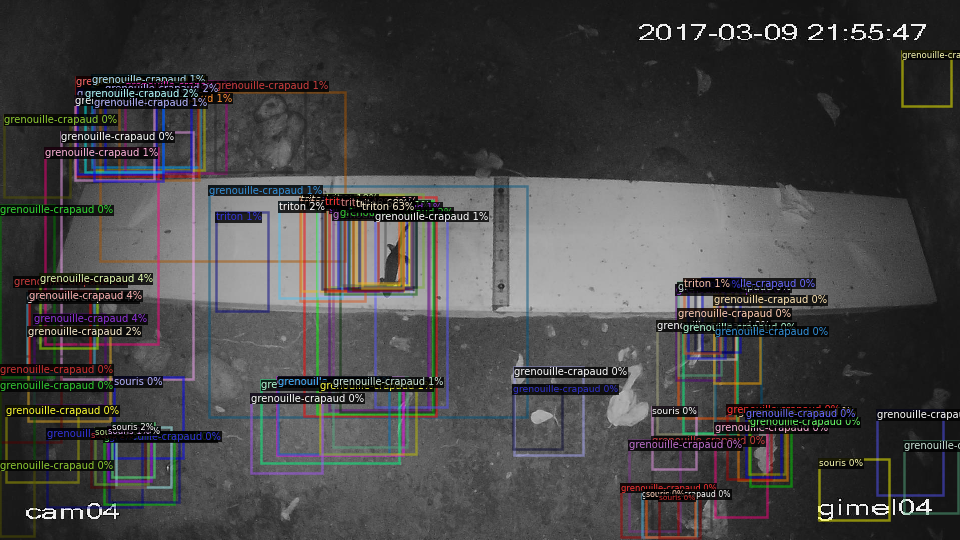
\includegraphics[width=\textwidth]{images/detr_threshold.png}
    \caption{Prédiction de DETR après un entrainement sur un GPU premium}
    \label{fig:detr_predictions_threshold}
\end{figure}

Nous pouvons observer que le triton au centre de l'image est correctement reconnu avec une probabilité de 63\% mais qu'il y a trop de bounding boxes. Nous voulions implémenter un système de filtrage après le modèle. Cependant nous n'avons pas réussis car le modèle ayant beaucoup de poids, il nécessitait un GPU puissant pour être entrainé. Nous avons déjà dépensé beaucoup d'argent de notre poche sur le service google colaboratory et nous n'avions pas les moyens de payer à nouveau pour entrainer et experimenter sur un GPU puissant. Nous avons donc abandonné l'idée de filtrer les bounding box. Vous pouvez néanmoins retrouver notre implémentation de DETR ici \url{https://colab.research.google.com/drive/1nJC4tI83L1_sLhfFUMZPk4bFN0Ui3Jfi?usp=sharing}. Une version ayant tourné une fois sur un GPU premium est disponible sur github sous le même nom.

Nous avons tenté une seconde implémentation de DETR en codant en PyTorch le modèle puisque on peut le faire en 60 lignes. L'entrainement était optimisé avec PyTorch Lightning. Nous avons réussis l'entrainement cependant en n'utilisant pas Detectron2, nous n'avons cette fois pas réussis à obtenir des scores sur le benchmark COCO fournit dans la class \verb|COCO_Evaluator| de Detectron2. Nous avons testé sur quelques images et voyons des bons résultats, de plus durant l'entrainement de bonnes métriques sont affichées cependant sans benchmark COCO, il est difficile de comparer ce modèle aux autres. Vous pouvez retrouver notre implémentation ici: \url{https://github.com/student-GML/crapauduc/blob/main/model_finaux/DETR_kaggle_fine_tune.ipynb}

En résumé : Nous n'avons pas réussis par manque de ressources à filtrer les probabilités faibles avec le wrapper Detectron2 de DETR. Nous avons cependant, avec PyTorch Lightning, réussis à avoir de bons scores durant l'entrainement. Ces résultats ne sont pas suffisants pour être comparés aux autres modèles. Et nous avons donc décider d'en rester là avec ce modèle.

\section{Modèles évalués}
D'après ces nombreuses recherches, nous avons donc implémenté et évaluer deux modèles fonctionnels dont nous avons pu comparer les scores d'évaluation sur des données tests : 

\begin{itemize}
    \item[-] Faster R-CNN avec Detectron2 ;
    \item[-] Retinanet avec Detectron2.
\end{itemize}